\chapter{Walidator}

Aplikacja posiada ograniczony zasób znanych osób oraz ich twarzy.
Jeżeli do aplikacji zostanie dostarczone zdjęcie osoby, która jest niezdefiniowana w systemie, klasyfikator SVM mimo
tego dokona klasyfikacji.
Owa sytuacja jest nieakceptowalna, ponieważ klasyfikator przeprowadzi wtedy zawsze błędną klasyfikację.
W celu rozwiązania problemu, przed dokonaniem klasyfikacji należy zweryfikować czy osoba,
która została przedstawiona na zdjęciu, jest znana systemowi.


\section{Odległości pomiędzy zdjęciami}

FaceNet został nauczony, aby mapować zdjęcia twarzy do zwartej przestrzeni euklidesowej.
Oznacza to, że odległości pomiędzy punktami odpowiadają mierze podobieństwa twarzy~\cite{schroff2015facenet}.
Jeżeli odległość jest mała, najprawdopodobniej zdjęcia przedstawiają tę samą osobę.

Po zaimportowaniu zdjęć z bazy~\cite{liu2015faceattributes} i wykonaniu zanurzenia (z ang. Embedding)
zostały zbadane odległości pomiędzy zdjęciami twarzy tych samych oraz różnych osób.
Wyniki zostały przedstawione w postaci histogramu na rysunku~\ref{fig:porownanie_histogramow_odleglosci}.

\begin{figure}[H]
    \centering
    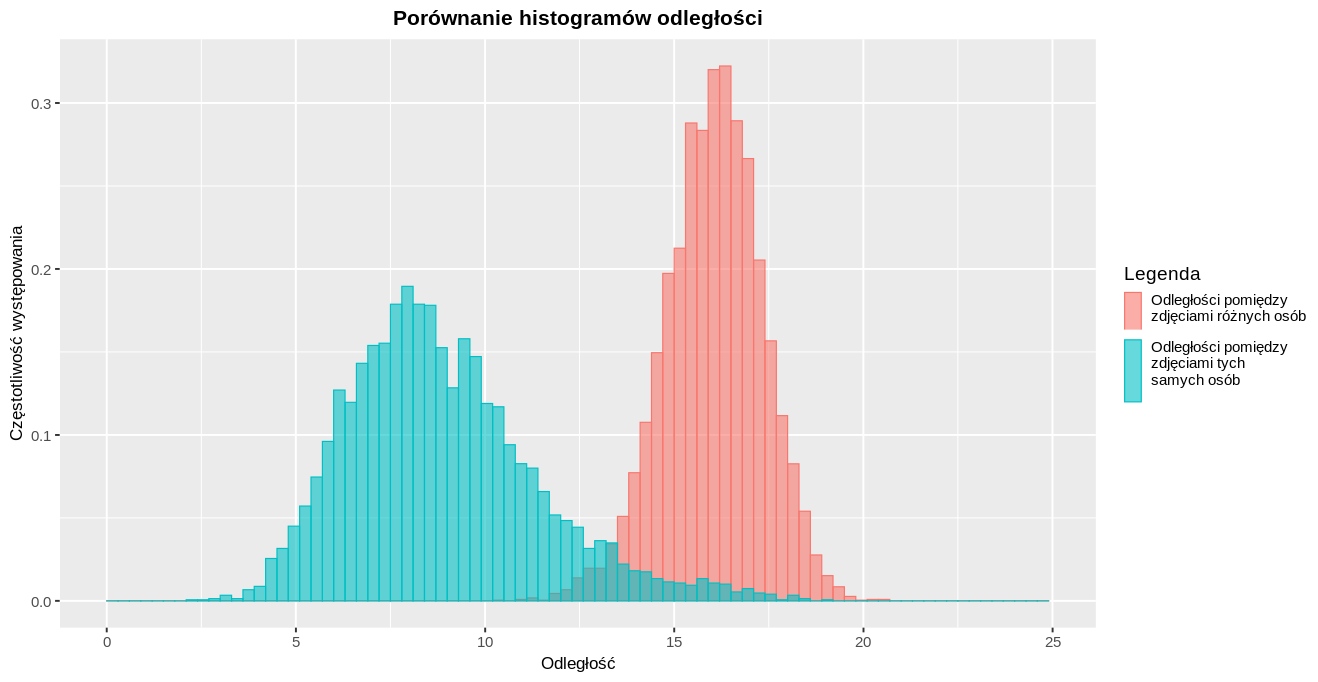
\includegraphics[width=1\textwidth]{./images/porownanie_histogramow_odleglosci}
    \caption{ Porównanie histogramów odległości pomiędzy zdjęciami twarzy tych samych oraz różnych osób }
    \customsource
    \label{fig:porownanie_histogramow_odleglosci}
\end{figure}

Z histogramu~\ref{fig:porownanie_histogramow_odleglosci} można odczytać, że w większości
przypadków odległość pomiędzy zdjęciami tej samej osoby jest
z przedziału od pięciu do trzynastu, natomiast dla zdjęć przedstawiających różne osoby od trzynastu do piętnastu.
Mając to na uwadze, można napisać funkcję, która będzie wyliczała, jaka jest odległość pomiędzy dostarczonym zdjęciem
a zdjęciami już umieszczonymi w bazie zdjęć.
Jeżeli odległość względem jakiegoś zdjęcia będzie mała, może to oznaczać, że dostarczone
zdjęcie \textbf{najprawdopodobniej} jest znane aplikacji.
W związku z tym, że funkcja będzie szukać najmniejszej odległości, nie ma potrzeby,
aby na histogramie~\ref{fig:porownanie_histogramow_odleglosci} wyświetlać wszystkie odległości.
Odległości, które mają największe znaczenie, to najmniejsze odległości pomiędzy dostarczonym zdjęciem
a zdjęciami danej etykiety.
Histogram z uwzględnieniem tylko najmniejszych odległości został przedstawiony na
rysunku~\ref{fig:wykres_najmniejszych_odleglosc_wspolny}.

\begin{figure}[H]
    \centering
    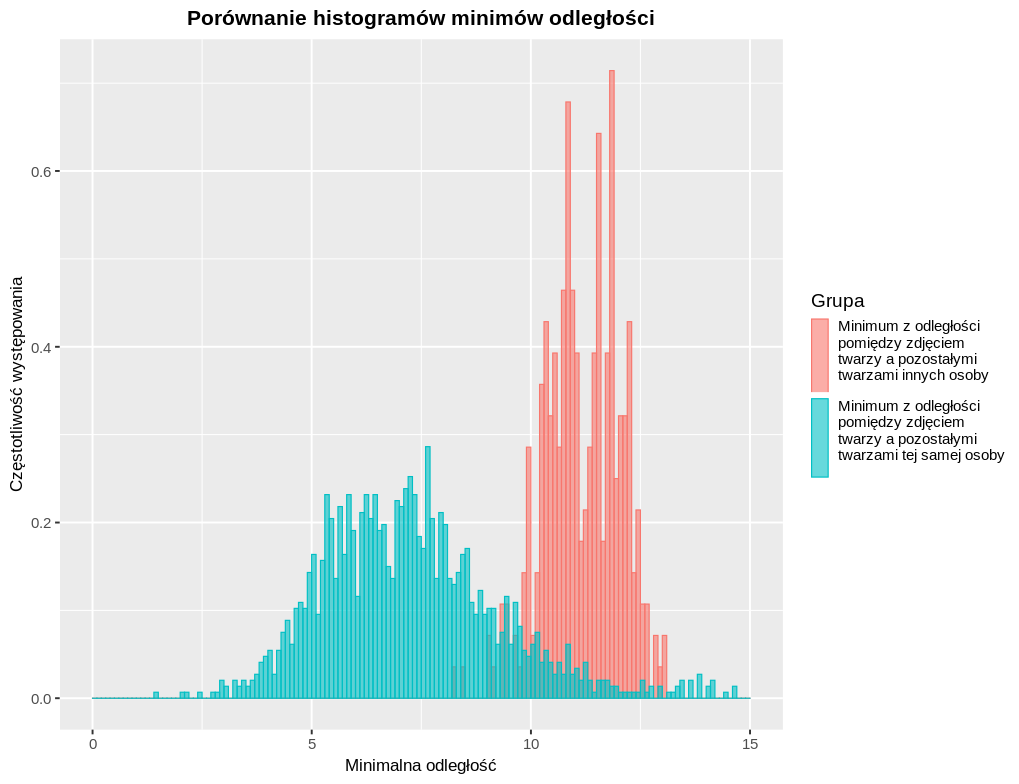
\includegraphics[width=1\textwidth]{images/wykres_najmniejszych_odleglosc_wspolny}
    \caption{
        Porównanie histogramów najmniejszych odległości pomiędzy
        zdjęciami twarzy tych samych oraz różnych osób.
    }
    \customsource
    \label{fig:wykres_najmniejszych_odleglosc_wspolny}
\end{figure}

Z wyników wykonanego badania wynika, że jeżeli do programu będą dostarczone zdjęcia przedstawiające osobę,
która została już dodana do systemu,
to odległość do najbliższego zdjęcia najprawdopodobniej będzie oscylować w przedziale od pięciu do dwunastu.


\section{Trafność walidatora}

W związku z tym, że

\begin{figure}[H]
    \centering
    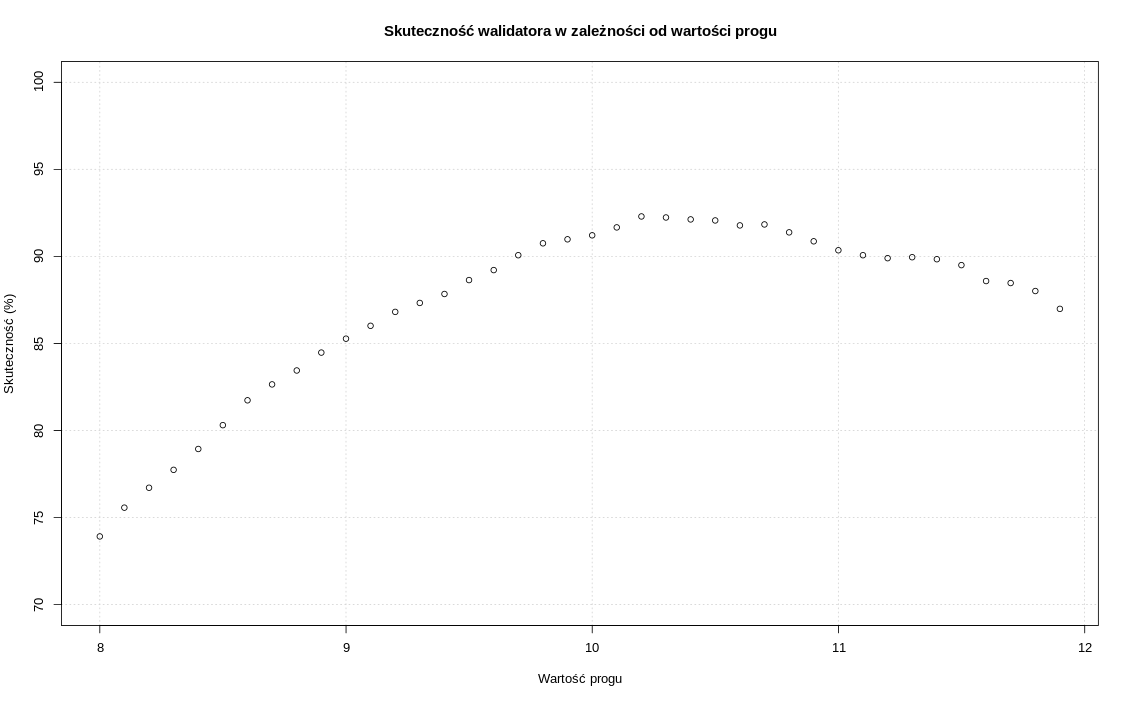
\includegraphics[width=1\textwidth]{images/trafnosc_walidator_a_prog}
    \caption{ Trafność walidatora w zależności od wartości progu }
    \customsource
    \label{fig:tranosc_walidatora_per_prog}
\end{figure}


\section{Wnioski}

Jeżeli walidator posluży do ...